% 原章第36页6.2.2起至第44页6.3标题前，式6.129—6.151。
\subsection{用于图像分割的监督深度学习方法}

分割是影像数据分析流程中的重要步骤（Litjens et al. 2017）。图像分割试图识别具有特定结构、图像空间变异与特征的体素集合。图像分割包括像素分割、实例分割和基于局部成分的分割（Garcia-Garcia et al. 2017）。卷积神经网络（CNN）与循环神经网络（recurrent neural network，RNN）这两类深度神经网络，广泛用于医学图像分割（Ronneberger et al. 2015；Xie et al. 2016）。像素层面的分割方法是各种分割的基础，本书重点讨论像素层面的分割。

\subsubsection{像素层面的图像分割}

像素层面的图像分割，根据图像特征为每个像素分配类别标签。CNN 常用于学习适合图像分割问题的特征表示，并已取得巨大成功（Ciresan et al. 2012；Farabet et al. 2013）。全卷积神经网络（fully convolutional neural network，FCNN）是一类常用的 CNN，能够有效生成特征，并采用端到端训练（Lin et al. 2016；Long et al. 2015）。FCNN 用于语义分割的局限是分辨率低。上下文关系广泛存在，但经典 CNN 尚未利用这类关系进行语义分割。近来，研究将图像区域之间的语义相关性引入 FCNN，利用条件随机场（conditional random field，CRF）预测图像像素的标签（Lin et al. 2016）。

\bookdeepheading{paragraph}{6.2.2.1.1}{用 CRF 建模语义成对关系}

CRF 是一种判别式无向概率图模型。考虑图 $G=(V,E)$，其中 $V$ 表示节点集，$E$ 表示边集。令 $X$ 为一组观测特征变量，$Y$ 为一组输出变量；给定观测特征变量 $X$，预测 $Y$（Sutton and McCallum 2011）。在利用 CRF 建模语义成对关系之前，先应用 CNN，从影像数据生成特征图（图 6.11a）。
\begin{figure}[htbp]
\centering
\begin{tikzpicture}[x=1cm,y=1cm,>=Stealth,font=\small]
\draw[green!65!black] (0,2.8)--(.7,3.4)--(.7,4.9)--(0,4.3)--cycle;
\node[red] at (.35,3.85) {图像};
\fill[yellow!85] (1.5,3.65) rectangle (3.2,4.25);\node[red] at (2.35,3.95) {CNN};
\draw[->,green!65!black] (.8,3.95)--(1.5,3.95);\draw[->,green!65!black] (3.2,3.95)--(4,3.95);
\draw[green!65!black] (4,2.8)--(4.8,3.5)--(4.8,5)--(4,4.2)--cycle;
\node[red] at (4.1,5.05) {特征图};\node[red] at (5.3,3.8) {CRF};
\draw[cyan!80!blue] (4.08,3.5)--(4.65,4.15) (4.25,3.48)--(4.25,4.2) (4.05,4.05)--(4.65,3.5) (4.16,3.72)--(4.58,3.74);
\foreach \xx/\yy in {4.22/3.7,4.55/3.72,4.52/4.2} \fill[red] (\xx,\yy) circle (2pt);
\node at (5.85,4.6) {节点};\draw[->,violet,dashed] (4.55,4.2)--(5.5,4.6);
\draw[cyan!80!blue] (6.1,3)--(6.1,3.7);\fill[red] (6.1,3) circle (2pt);\fill[red] (6.1,3.7) circle (2pt);
\node at (6,2.65) {CRF 图中的边（连接）};\draw[->,violet,dashed] (5.4,2.8)--(6.1,3.35);
\node at (-.3,2.75) {(a)};
\filldraw[fill=green!70!black,draw=magenta,dashed] (0,1) rectangle (1.9,2.4);
\draw[yellow] (.55,1.45)--(1,1.85);\fill[red] (.55,1.45) circle (3pt);\fill[red] (1,1.85) circle (3pt);
\filldraw[fill=green!70!black,draw=magenta,dashed] (2.3,.95) rectangle (4.2,2.35);
\draw[violet] (2.7,1.8)--(3.25,1.1)--(3.75,1.9);
\foreach \xx/\yy in {2.7/1.8,3.25/1.1,3.75/1.9} \fill[red] (\xx,\yy) circle (3pt);
\node at (-.3,.9) {(b)};
\draw[green!65!black] (4.55,1.35) rectangle (5.1,2);
\fill[red] (4.82,1.55) circle (2pt);\fill[red] (4.82,1.87) circle (2pt);
\draw[->,red,dashed] (4.55,3.72)--(4.82,2);
\fill[yellow!85] (5.5,.9) rectangle (6.8,2.25);\node[red,align=center] at (6.15,1.58) {全连接\\层};
\foreach \yy in {.9,1.3,1.65,2.25} \draw[->,green!65!black] (5.1,1.65)--(5.5,\yy);
\foreach \yy in {.95,1.6,2.1} \draw[->,magenta] (6.8,1.6)--(7.1,\yy);
\node[magenta,anchor=west] at (6.95,2.3) {$K\times K$};\node[magenta,anchor=west] at (7.15,1.6) {类别};
\node at (4.55,.8) {(c)};
\end{tikzpicture}
\origfig{11}{CRF 模型。（a）使用 CNN 从影像数据生成特征图；（b）空间范围框；（c）成对网络。}
\end{figure}


特征图中的每个神经元（位置）由 CRF 图中的一个节点表示；它还与同一空间范围框（图 6.11b 中粉色虚线框）内的其他全部节点相连（Lin et al. 2016）。空间关系不同，就定义不同的空间范围框，并用不同的边建模不同的空间关系（图 6.11b 中黄色边与紫色边）。为降低模型中数据的维数，可定义与每个节点及每条边关联的特征向量。

接着定义图上的分布，使其考虑输入—输出对的相容性（Lin et al. 2016）。给定输入图像记为 $x$，其逐像素标签记为 $y$。令 $X=\{x\}$ 为影像数据集，$Y=\{y\}$ 为标签集；它们对应 CRF 各节点的标签配置。令 $V=X\cup Y$。先定义给定 $x$ 时 $y$ 的条件分布 $P(y\mid x)$。令 $E(y,x,\theta)$ 为能量函数，度量输入—输出对的相容性。CRF 的全部参数记为 $\theta$。一幅图像的条件分布定义为
\begin{equation}
p(y\mid x)=\frac1{Z(x)}e^{-E(y,x)}.
\tag{6.129}
\end{equation}
由于 $\sum_yp(y\mid x)=1$，要求 $Z(x)=\sum_ye^{-E(y,x)}$，函数 $Z(x)$ 称为配分函数（partition function）。

下面定义能量函数。CRF 是一个因子图 $G$，因此条件分布应按 $G$ 分解：
\begin{equation}
p(y\mid x)=\frac1{Z(x)}\prod_{\alpha=1}^A\Psi_{\alpha}(y_{\alpha},x_{\alpha}),
\tag{6.130}
\end{equation}
其中，$\Psi_{\alpha}(y_{\alpha},x_{\alpha})$ 通常称为势函数（potential function），具有指数形式：
\begin{equation}
\Psi_{\alpha}(y_{\alpha},x_{\alpha})=e^{-E(y_{\alpha},x_{\alpha})}.
\tag{6.131}
\end{equation}
势函数集 $A$ 可分为一元势函数集与成对势函数集两个子集（Lin et al. 2016）。

为计算一元势函数，先将特征图与一个浅层全连接网络堆叠起来。这个全连接网络也称为一元网络（unary-net），其输出可作为一元势函数。令 $K$ 为类别数，一元网络节点的输出是 $K$ 维向量。一元网络中第 $p$ 个节点、第 $y_p$ 类的一元势函数定义为
\begin{equation}
U(y_p,x_p;\theta_U)=-\beta_{p,y_p}(x;\theta_U),
\tag{6.132}
\end{equation}
其中，$\beta_{p,y_p}$ 为一元网络第 $p$ 个节点、第 $y_p$ 类的输出值，$\theta_U$ 为一元网络 $U$ 中的参数集。令 $A_U$ 为全部一元势的集合，$N_U$ 为势 $U$ 的节点集，则一元势的能量函数定义为
\begin{equation}
E_U(y,x,\theta)=\sum_{U\in A_U}\sum_{p\in N_U}U(y_p,x_p;\theta_U).
\tag{6.133}
\end{equation}
接着研究成对势函数。考虑 CRF 图中相连的两个节点 $p$ 与 $q$。令 $x_p,x_q$ 分别为节点 $p,q$ 的特征向量，均来自特征图。令 $x_{pq}=[x_p^T,x_q^T]^T$ 为边特征向量。随后将边特征向量 $x_{pg}$ 输入一个称为成对网络（pairwise-net）的全连接网络（图 6.11c）。类别总数为 $K\times K$，即一对节点所有可能的标签组合数。成对网络预测的类别记为 $(y_p,y_q)$。令 $\beta_{p,q,y_p,y_q}(x;\theta_V)$ 为成对网络中对应 $x_{pq}$ 的输出值，量化输入影像数据 $x$ 下类别 $(y_p,y_q)$ 的相容性。节点对 $p,q$ 的成对势函数定义为
\begin{equation}
V(y_p,y_q,x_{pq},\theta_V)=-\beta_{p,q,y_p,y_q}(x;\theta_V),
\tag{6.134}
\end{equation}
其中，$\theta_V$ 为定义势 $V$ 的 CNN 参数。令 $A_V$ 为所有成对势类型的集合，$\varepsilon_V$ 为计算成对势 $V$ 所用的边集。一组成对势的能量函数定义为
\begin{equation}
E_V(y,x,\theta)=\sum_{V\in A_V}\sum_{(p,q)\in\varepsilon_V}V(y_p,y_q,x_{pq},\theta_V).
\tag{6.135}
\end{equation}
总能量函数由一组一元势与成对势定义：
\begin{equation}
E(y,x,\theta)=E_U(y,x,\theta)+E_V(y,x,\theta).
\tag{6.136}
\end{equation}

\bookdeepheading{paragraph}{6.2.2.1.2}{CRF 模型的参数估计}

负对数似然可用于估计 CRF 模型参数。由式 (6.129)，一幅图像的负对数似然为
\begin{equation}
-\log p(y\mid x,\theta)=E(y,x,\theta)+\log Z(x,\theta).
\tag{6.137}
\end{equation}
假定从训练集中抽取 $N$ 幅图像，令 $x_i,y_i$ 为第 $i$ 幅图像中像素的影像信号与标签，则 $N$ 幅图像的负对数似然为
\begin{equation}
-\sum_{i=1}^N\log P(y^{(i)}\mid x^{(i)},\theta)=\sum_{i=1}^N[E(y^{(i)},x^{(i)},\theta)+\log Z(x^{(i)},\theta)].
\tag{6.138}
\end{equation}
为提高效率与预测精度，应减少模型参数。因此，在式 (6.137) 的负似然中加入参数惩罚项，最终将参数估计问题化为
\begin{equation}
\min_{\theta}l(y,x,\theta)=\sum_{i=1}^N[E(y^{(i)},x^{(i)},\theta)+\log Z(x^{(i)},\theta)]+\frac\lambda2\lVert\theta\rVert_2^2.
\tag{6.139}
\end{equation}
精确的极大似然估计需要反复直接计算 $Z(x,\theta)$ 及其偏导数，计算代价很高，因此需要发展 CRF 的近似学习方法。常用方法包括伪似然学习（pseudo-likelihood learning）与分片学习（piecewise learning）（Besag 1977；Sutton and McCallum 2005；Lin et al. 2016）。本节重点介绍分片学习。其基本思想是，将整个模型（图）分为若干片段（子图），各自独立学习，最后在测试时组合各子模型学到的权重。假定定义一元势的节点集，以及定义成对势的边（节点）集，分别形成片段。为每个片段定义似然，并将这些似然视为相互独立。整个模型的条件似然可用这些片段独立似然的乘积近似（Lin et al. 2016）：
\begin{equation}
P(y\mid x)=\prod_{U\in A_U}\prod_{p\in N_U}P_U(y_p\mid x)\prod_{V\in A_V}\prod_{(p,q)\in\varepsilon_V}P_V(y_p,y_q\mid x),
\tag{6.140}
\end{equation}
其中，似然 $P_U(y_p\mid x)$ 由一元势定义：
\begin{equation}
P_U(y_p\mid x)=\frac{\exp\{-U(y_p,x_p)\}}{\displaystyle\sum_{y_h}\exp\{-U(y_h,x_h)\}},
\tag{6.141}
\end{equation}
似然 $P_V(y_p,y_q\mid x)$ 由成对势定义：
\begin{equation}
P_V(y_p,y_q\mid x)=\frac{\exp\{-V(y_p,y_q,x_{pq})\}}{\displaystyle\sum_{y_g,y_h}\exp\{-V(y_g,y_h,x_{gh})\}}.
\tag{6.142}
\end{equation}
利用式 (6.140) 对似然作分片近似后，参数估计优化问题 (6.139) 化为（Lin et al. 2016）
\begin{equation}
\begin{aligned}
\min_{\theta}l_a(y,x,\theta)&=-\sum_{i=1}^N\Biggl[\sum_{U\in A_U}\sum_{p\in N_U^{(i)}}\log P_U(y_p\mid x^{(i)},\theta_U)\\
&\qquad+\sum_{V\in A_V}\sum_{(p,q)\in\varepsilon_V^{(i)}}\log P_V(y_p,y_q\mid x^{(i)},\theta_V)\Biggr]+\frac\lambda2\lVert\theta\rVert_2^2.
\end{aligned}\tag{6.143}
\end{equation}
式 (6.143) 的目标函数是独立对数似然之和，因此优化问题 (6.143) 很容易并行求解。

\bookdeepheading{paragraph}{6.2.2.1.3}{预测}

可通过最大化后验分布 $y^*=\arg\max_yP(y\mid x)$，预测一个像素的类别标签；也可计算每个变量标签的边缘分布，即对所有 $p\in N$ 计算
\begin{equation}
P(y_p\mid x)=\sum_{y\setminus y_p}P(y\mid x),
\tag{6.144}
\end{equation}
其中，$y\setminus y_p$ 表示除 $y_p$ 外的输出类别变量 $y$。直接计算边缘分布在计算上不可行，需要近似方法。常用的近似概率推断方法是平均场方法（mean field method）：在可处理的分布子集中，寻找最能近似分布 $P(y\mid x,\theta)$ 的分布（Nowozin and Lampert 2011）。

Kullback–Leibler（K–L）散度是广泛使用的两分布间距离度量。令 $\Omega$ 为 $Y$ 上一族可处理的分布 $q\in\Omega$。定义分布 $q$ 与 $P(y\mid x,\theta)$ 之间的 K–L 散度 $D^{\mathrm{KL}}$ 为
\begin{equation}
D_{\mathrm{KL}}(q(y)\Vert P(y\mid x,\theta)=\sum_{y\in Y}q(y)\log\frac{q(y)}{P(y,x,\theta)}.
\tag{6.145}
\end{equation}
我们的目标是求解以下优化问题，得到最佳近似分布 $q(y)$：
\begin{equation}
\min_{q\in\Omega}D_{\mathrm{KL}}(q(y)\Vert P(y\mid x,\theta)).
\tag{6.146}
\end{equation}
回顾，边缘分布 $P(y\mid x,\theta)$ 可表示为
\begin{equation}
P(y\mid x,\theta)=\frac1{Z(x,\theta)}e^{-E(y,x,\theta)},
\tag{6.147}
\end{equation}
其中，$E(y,x,\theta)$ 为能量函数。利用图模型，大量随机变量上的分布可表示为若干局部函数的乘积，每个局部函数只依赖少数变量。假定 $\Omega$ 由全部因子化分布构成，即
\[
q(y)=\prod_{i\in V}q_i(y_i).
\]
利用朴素平均场方法，可在分布集 $\Omega$ 中得到最佳近似分布（附录 6.A）：
\begin{equation}
\begin{aligned}
\widehat q_i(y_i)=\exp\Biggl(&\lambda-1-\sum_{a\in F,i\in N(a)}\sum_{\substack{y_{N(a)}\in Y_{N(a)},\\{}[y_{N(a)}]=y_i}}\\
&\left(\prod_{j\in N(a)\setminus\{i\}}\widehat q_j(y_j)\right)E_a(y_{N(a)},x_{N(a)})\Biggr),
\end{aligned}\tag{6.148}
\end{equation}
其中
\begin{equation}
\begin{aligned}
\lambda=-\log\Biggl(\sum_{y_i\in Y_i}\exp\Biggl(&-1-\sum_{a\in F,i\in N(a)}\sum_{\substack{y_{N(a)}\in Y_{N(a)},\\{}[y_{N(a)}]=y_i}}\\
&\left(\prod_{j\in N(a)\setminus\{i\}}\widehat q_j(y_j)\right)E_a(y_{N(a)},x_{N(a)})\Biggr)\Biggr).
\end{aligned}\tag{6.149}
\end{equation}
对各个 $i\in V$ 更新 $q_i(y_i)$，将收敛到优化问题 (6.146) 的解。

\subsubsection{用于语义分割的反卷积网络}

用于语义分割的全卷积网络（fully convolutional network，FCN）有一些局限（Noh et al. 2015）。第一，即使对象较大，像素标签预测也仅使用位置信息，导致同一对象中像素的标签预测不一致。第二，反卷积过程过于简单，常会丢失对象的空间变异信息与语义分割结构。为克服这些局限，研究发展了反卷积网络（deconvolution network）（Noh et al. 2015；Zeiler et al. 2011）。反卷积网络由反卷积、反池化与修正构成。卷积网络通过前馈减小激活尺寸，而反卷积网络中反池化与反卷积的组合可增大激活尺寸（Zeiler et al. 2011）。反卷积网络的任务，是从卷积网络生成的特征产生语义分割。其最终输出为每个像素的标签概率图，大小与输入图像相同。

\bookdeepheading{paragraph}{6.2.2.2.1}{反池化}

卷积网络池化层的作用，是在感受野内取最大激活，用一个值滤除含噪激活，因而会丢失空间变异信息（Noh et al. 2015）。
\begin{figure}[htbp]
\centering
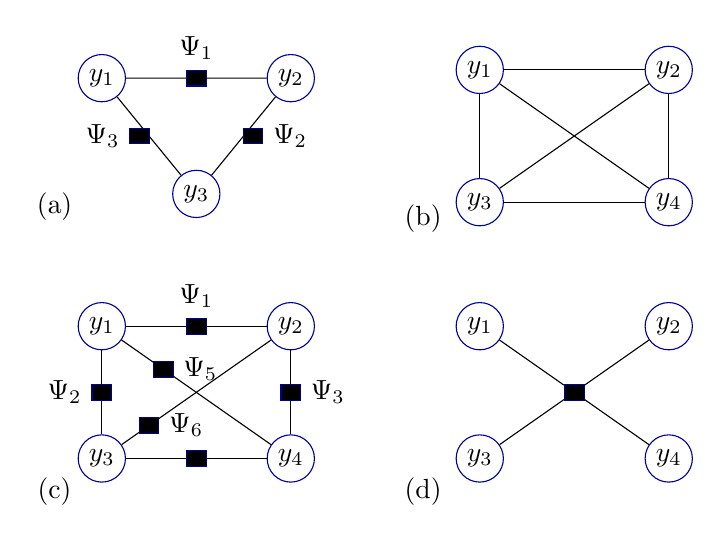
\begin{tikzpicture}[x=1.2cm,y=1.05cm,
chSixFtwelveV/.style={circle,draw=blue!60!black,fill=white,minimum size=6mm,inner sep=1pt},
chSixFtwelveF/.style={rectangle,fill=black,draw=blue!60!black,minimum width=2.5mm,minimum height=2mm,inner sep=0pt}]
\node[chSixFtwelveV] (chSixF12a1) at (0,4) {$y_1$};\node[chSixFtwelveV] (chSixF12a2) at (2,4) {$y_2$};\node[chSixFtwelveV] (chSixF12a3) at (1,2.6) {$y_3$};
\draw (chSixF12a1)--(chSixF12a2)--(chSixF12a3)--(chSixF12a1);
\node[chSixFtwelveF,label=above:$\Psi_1$] at (1,4) {};\node[chSixFtwelveF,label=right:$\Psi_2$] at (1.6,3.3) {};\node[chSixFtwelveF,label=left:$\Psi_3$] at (.4,3.3) {};
\node at (-.5,2.45) {(a)};
\foreach \nn/\xx/\yy in {1/4/4.1,2/6/4.1,3/4/2.5,4/6/2.5}
 \node[chSixFtwelveV] (chSixF12b\nn) at (\xx,\yy) {$y_{\nn}$};
\foreach \aa/\bb in {1/2,1/3,1/4,2/3,2/4,3/4} \draw (chSixF12b\aa)--(chSixF12b\bb);
\node at (3.4,2.3) {(b)};
\foreach \nn/\xx/\yy in {1/0/1,2/2/1,3/0/-.6,4/2/-.6}
 \node[chSixFtwelveV] (chSixF12c\nn) at (\xx,\yy) {$y_{\nn}$};
\foreach \aa/\bb in {1/2,1/3,1/4,2/3,2/4,3/4} \draw (chSixF12c\aa)--(chSixF12c\bb);
\node[chSixFtwelveF,label=above:$\Psi_1$] at (1,1) {};
\node[chSixFtwelveF,label=left:$\Psi_2$] at (0,.2) {};
\node[chSixFtwelveF,label=right:$\Psi_3$] at (2,.2) {};
\node[chSixFtwelveF] at (1,-.6) {};
\node[chSixFtwelveF,label=right:$\Psi_5$] at (.65,.48) {};
\node[chSixFtwelveF,label=right:$\Psi_6$] at (.5,-.2) {};
\node at (-.5,-1) {(c)};
\foreach \nn/\xx/\yy in {1/4/1,2/6/1,3/4/-.6,4/6/-.6}
 \node[chSixFtwelveV] (chSixF12d\nn) at (\xx,\yy) {$y_{\nn}$};
\node[chSixFtwelveF] (chSixF12df) at (5,.2) {};
\foreach \nn in {1,2,3,4} \draw (chSixF12d\nn)--(chSixF12df);
\node at (3.4,-1) {(d)};
\end{tikzpicture}
\origfig{12}{因子图。（a）三个变量上的因子图（引文见例 A1）；（b）具有完全连接图的马尔可夫随机场（引文见例 A2）；（c）该马尔可夫随机场的一种可能因子分解（引文见例 A2）；（d）一个因子图（引文见习题 5）。}
\end{figure}


反池化（unpooling）是一种恢复丢失的空间变异信息的逆向运算。卷积生成特征图后（图 6.13a），对特征图执行池化，在感受野内取最大特征，得到池化图及位置（开关）；后者记录绝对特征最大值的位置（图 6.13b）。沿相反方向，给定池化运算的对应位置信息，反池化在池化开关记录的位置插入特征值，形成反池化特征图（图 6.13c）。然后，将反池化特征与核卷积（图 6.13d）。
\begin{figure}[htbp]
\centering
\begin{tikzpicture}[x=1cm,y=1cm,>=Stealth,font=\small]
\filldraw[fill=cyan!20,draw=white] (0.0,5.1) rectangle ++(0.72,-0.4);
\node[text=red,font=\small] at (0.36,4.8999999999999995) {-1};
\filldraw[fill=cyan!20,draw=white] (0.72,5.1) rectangle ++(0.72,-0.4);
\node[text=green!65!black,font=\small] at (1.08,4.8999999999999995) {1};
\filldraw[fill=cyan!20,draw=white] (0.0,4.699999999999999) rectangle ++(0.72,-0.4);
\node[text=blue!70!black,font=\small] at (0.36,4.5) {1.2};
\filldraw[fill=cyan!20,draw=white] (0.72,4.699999999999999) rectangle ++(0.72,-0.4);
\node[text=magenta,font=\small] at (1.08,4.5) {0.9};\filldraw[fill=cyan!20,draw=white] (2.25,5.1) rectangle ++(0.85,-0.4);
\node[text=red,font=\small] at (2.675,4.8999999999999995) {1,3};
\filldraw[fill=cyan!20,draw=white] (3.1,5.1) rectangle ++(0.85,-0.4);
\node[text=green!65!black,font=\small] at (3.525,4.8999999999999995) {2,1};
\filldraw[fill=cyan!20,draw=white] (2.25,4.699999999999999) rectangle ++(0.85,-0.4);
\node[text=blue!70!black,font=\small] at (2.675,4.5) {3,4};
\filldraw[fill=cyan!20,draw=white] (3.1,4.699999999999999) rectangle ++(0.85,-0.4);
\node[text=magenta,font=\small] at (3.525,4.5) {4,2};\filldraw[fill=cyan!20,draw=white] (7.2,5.1) rectangle ++(0.72,-0.4);
\node[text=red,font=\small] at (7.5600000000000005,4.8999999999999995) {1};
\filldraw[fill=cyan!20,draw=white] (7.92,5.1) rectangle ++(0.72,-0.4);
\node[text=green!65!black,font=\small] at (8.280000000000001,4.8999999999999995) {2};
\filldraw[fill=cyan!20,draw=white] (7.2,4.699999999999999) rectangle ++(0.72,-0.4);
\node[text=blue!70!black,font=\small] at (7.5600000000000005,4.5) {3};
\filldraw[fill=cyan!20,draw=white] (7.92,4.699999999999999) rectangle ++(0.72,-0.4);
\node[text=magenta,font=\small] at (8.280000000000001,4.5) {4};\filldraw[fill=cyan!20,draw=white] (0.0,3.5) rectangle ++(0.72,-0.4);
\node[text=red,font=\small] at (0.36,3.3) {02};
\filldraw[fill=cyan!20,draw=white] (0.72,3.5) rectangle ++(0.72,-0.4);
\node[text=red,font=\small] at (1.08,3.3) {0.3};
\filldraw[fill=cyan!20,draw=white] (1.44,3.5) rectangle ++(0.72,-0.4);
\node[text=green!65!black,font=\small] at (1.7999999999999998,3.3) {1};
\filldraw[fill=cyan!20,draw=white] (2.16,3.5) rectangle ++(0.72,-0.4);
\node[text=green!65!black,font=\small] at (2.52,3.3) {0.5};
\filldraw[fill=cyan!20,draw=white] (0.0,3.1) rectangle ++(0.72,-0.4);
\node[text=red,font=\small] at (0.36,2.9) {-1};
\filldraw[fill=cyan!20,draw=white] (0.72,3.1) rectangle ++(0.72,-0.4);
\node[text=red,font=\small] at (1.08,2.9) {0.8};
\filldraw[fill=cyan!20,draw=white] (1.44,3.1) rectangle ++(0.72,-0.4);
\node[text=green!65!black,font=\small] at (1.7999999999999998,2.9) {0.4};
\filldraw[fill=cyan!20,draw=white] (2.16,3.1) rectangle ++(0.72,-0.4);
\node[text=green!65!black,font=\small] at (2.52,2.9) {0.8};
\filldraw[fill=cyan!20,draw=white] (0.0,2.7) rectangle ++(0.72,-0.4);
\node[text=blue!70!black,font=\small] at (0.36,2.5) {0};
\filldraw[fill=cyan!20,draw=white] (0.72,2.7) rectangle ++(0.72,-0.4);
\node[text=blue!70!black,font=\small] at (1.08,2.5) {0.7};
\filldraw[fill=cyan!20,draw=white] (1.44,2.7) rectangle ++(0.72,-0.4);
\node[text=magenta,font=\small] at (1.7999999999999998,2.5) {0.5};
\filldraw[fill=cyan!20,draw=white] (2.16,2.7) rectangle ++(0.72,-0.4);
\node[text=magenta,font=\small] at (2.52,2.5) {0.9};
\filldraw[fill=cyan!20,draw=white] (0.0,2.3) rectangle ++(0.72,-0.4);
\node[text=blue!70!black,font=\small] at (0.36,2.0999999999999996) {0.2};
\filldraw[fill=cyan!20,draw=white] (0.72,2.3) rectangle ++(0.72,-0.4);
\node[text=blue!70!black,font=\small] at (1.08,2.0999999999999996) {1.2};
\filldraw[fill=cyan!20,draw=white] (1.44,2.3) rectangle ++(0.72,-0.4);
\node[text=magenta,font=\small] at (1.7999999999999998,2.0999999999999996) {0.1};
\filldraw[fill=cyan!20,draw=white] (2.16,2.3) rectangle ++(0.72,-0.4);
\node[text=magenta,font=\small] at (2.52,2.0999999999999996) {0.8};\filldraw[fill=cyan!20,draw=white] (6.6,3.5) rectangle ++(0.72,-0.4);
\node[text=red,font=\small] at (6.96,3.3) {0};
\filldraw[fill=cyan!20,draw=white] (7.319999999999999,3.5) rectangle ++(0.72,-0.4);
\node[text=red,font=\small] at (7.68,3.3) {0};
\filldraw[fill=cyan!20,draw=white] (8.04,3.5) rectangle ++(0.72,-0.4);
\node[text=green!65!black,font=\small] at (8.399999999999999,3.3) {2};
\filldraw[fill=cyan!20,draw=white] (8.76,3.5) rectangle ++(0.72,-0.4);
\node[text=green!65!black,font=\small] at (9.12,3.3) {0};
\filldraw[fill=cyan!20,draw=white] (6.6,3.1) rectangle ++(0.72,-0.4);
\node[text=red,font=\small] at (6.96,2.9) {1};
\filldraw[fill=cyan!20,draw=white] (7.319999999999999,3.1) rectangle ++(0.72,-0.4);
\node[text=red,font=\small] at (7.68,2.9) {0};
\filldraw[fill=cyan!20,draw=white] (8.04,3.1) rectangle ++(0.72,-0.4);
\node[text=green!65!black,font=\small] at (8.399999999999999,2.9) {0};
\filldraw[fill=cyan!20,draw=white] (8.76,3.1) rectangle ++(0.72,-0.4);
\node[text=green!65!black,font=\small] at (9.12,2.9) {0};
\filldraw[fill=cyan!20,draw=white] (6.6,2.7) rectangle ++(0.72,-0.4);
\node[text=blue!70!black,font=\small] at (6.96,2.5) {0};
\filldraw[fill=cyan!20,draw=white] (7.319999999999999,2.7) rectangle ++(0.72,-0.4);
\node[text=blue!70!black,font=\small] at (7.68,2.5) {0};
\filldraw[fill=cyan!20,draw=white] (8.04,2.7) rectangle ++(0.72,-0.4);
\node[text=magenta,font=\small] at (8.399999999999999,2.5) {0};
\filldraw[fill=cyan!20,draw=white] (8.76,2.7) rectangle ++(0.72,-0.4);
\node[text=magenta,font=\small] at (9.12,2.5) {4};
\filldraw[fill=cyan!20,draw=white] (6.6,2.3) rectangle ++(0.72,-0.4);
\node[text=blue!70!black,font=\small] at (6.96,2.0999999999999996) {0};
\filldraw[fill=cyan!20,draw=white] (7.319999999999999,2.3) rectangle ++(0.72,-0.4);
\node[text=blue!70!black,font=\small] at (7.68,2.0999999999999996) {3};
\filldraw[fill=cyan!20,draw=white] (8.04,2.3) rectangle ++(0.72,-0.4);
\node[text=magenta,font=\small] at (8.399999999999999,2.0999999999999996) {0};
\filldraw[fill=cyan!20,draw=white] (8.76,2.3) rectangle ++(0.72,-0.4);
\node[text=magenta,font=\small] at (9.12,2.0999999999999996) {0};
\node at (.72,5.4) {池化图};\node at (3.1,5.4) {位置（开关）};\node at (7.92,5.4) {输入};
\node at (2.6,3.8) {特征图};\node at (8.8,3.8) {反池化};
\node[anchor=east] at (.45,3.9) {池化};\draw[->,green!65!black,line width=1pt] (.72,3.5)--(.72,4.3);
\node[anchor=east] at (6.5,4) {反池化};\draw[->,green!65!black,line width=1pt] (6.85,4.4)--(6.85,3.5);
\fill[green!60] (-.15,-.4) rectangle (3.95,1.4);\node[red] at (1.9,.5) {卷积};
\fill[yellow!85] (6.2,-.4) rectangle (10.3,1.4);\node[red] at (8.25,.5) {反卷积};
\draw[->,green!65!black,line width=1pt] (1.9,1.4)--(1.9,1.9);
\draw[->,green!65!black,line width=1pt] (8.1,1.9)--(8.1,1.4);
\node at (-.3,1.75) {(b)};\node at (6,1.75) {(c)};\node at (-.3,-.65) {(a)};\node at (6,-.65) {(d)};
\end{tikzpicture}
\origfig{13}{反池化与反卷积。（a）卷积生成特征图；（b）对特征图执行池化；（c）反池化特征图；（d）对反池化特征进行反卷积。}
\end{figure}


\bookdeepheading{paragraph}{6.2.2.2.2}{反卷积}

反卷积层将反池化特征与多个已学习的核卷积，产生多个输出。令 $K_l$ 为第 $l$ 个反卷积层的核数目，$f_{k,m}^l$ 为第 $l$ 层中与前一层第 $m$ 个特征图卷积的第 $k$ 个核，$z_{k,l}$ 为第 $l-1$ 个反卷积层中的反池化特征与核 $f_{k,l}$ 卷积的输出，则
\begin{equation}
z_{k,l}=z_{m,l-1}*f_{k,m}^l,\quad k=1,2,\ldots,K_l,
\tag{6.150}
\end{equation}
其中，$z_{l-1}$ 为第 $l-1$ 个反卷积层的反池化特征。因此，反卷积层的输出是尺寸增大的稠密激活图。

\bookdeepheading{paragraph}{6.2.2.2.3}{模型与参数估计}

为建立用于推断参数的代价函数，考虑第 $l$ 个反卷积网络层（Zeiler et al. 2010）。设图像集为 $y=\{y^1,\ldots,y^N\}$，其中 $N$ 为图像数目。考虑第 $i$ 幅图像 $y^i$，令 $z_{k,l}^i$ 为第 $l$ 个反卷积层的特征图，作为带核 $f_{k,m}^l$ 的第 $l-1$ 个反卷积层的输入；$z_{m,l-1}^i$ 为前一个即第 $l-1$ 个反卷积层的特征图。令 $K_{l-1}$ 与 $K_l$ 分别为第 $l$ 层和第 $l-1$ 层的特征图数目。定义第 $l$ 层的代价函数 $C_l(y)$ 为
\begin{equation}
\begin{aligned}
C_l(y)&=\frac12\sum_{i=1}^N\sum_{m=1}^{K_{l-1}}\left\lVert\sum_{k=1}^{K_l}h_{k,m}^l(z_{k,l}^i*f_{k,m}^l)-z_{m,l-1}^i\right\rVert_2^2\\
&\quad+\lambda\sum_{i=1}^N\sum_{k=1}^{K_l}\lVert z_{k,l}^1\rVert_1,
\end{aligned}\tag{6.151}
\end{equation}
其中，$\lambda$ 为惩罚参数，$h_{k,m}^l$ 为指示矩阵元素，定义为
\[
h_{k,m}^l=\begin{cases}1,&\text{若 }z_{k,l}^i\text{ 与 }z_{m,l-1}^i\text{ 相连},\\0,&\text{其他情形}.\end{cases}
\]
在第一层，假定对所有 $k,m$ 均有 $h_{k,m}^l=1$。

代价函数 $C_l(y)$ 包含两项：（1）重构误差；（2）正则化项。学习的目标是使重构误差尽可能小，正则化项则惩罚估计的特征值。这两个目标相互冲突，惩罚参数 $\lambda$ 用于平衡两者。

通过对特征图中的激活量 $z_{k,m}^l$ 与核函数 $f_{k,m}^l$，极小化式 (6.150) 中的代价函数 $C_l(y)$，可估计反卷积网络参数。交替方向乘子法（ADMM）与近端方法（Boyd et al. 2011；Parikh and Boyd 2014）可用于求解该问题。
